
%================================================================


　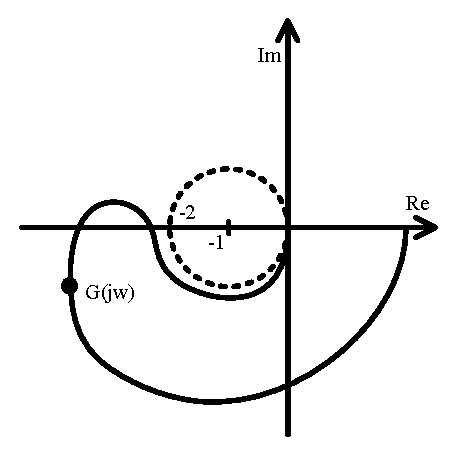
\epsfig{file=92others/nyquist_prob.eps,scale=0.6}


\vspace{-2cm}
%================================================================
\item
Riccati方程式を変形することにより最適制御の一巡伝達関数$G(s)$が$|1+ G(j\omega)|>1$を満たすことが証明できる．これを用いて以下の問いに答えよ．
\begin{enumerate}
\item
この条件を満たす$G(j\omega)$のベクトル軌跡は下図のようになる．$1+G(j \omega)$のベクトルを図に記入し，このベクトル軌跡を説明せよ．（下図は元のシステムが安定である場合を示している）
\vspace{5cm}
\item
最適制御のゲイン余裕は$1/2$から$\infty$である（入力のゲインが$1/2$〜$\infty$まで変化しても閉ループ系の安定性が保たれる）ことを説明せよ．
\end{enumerate}
%================================================================
